\documentclass{TDP005mall}



\newcommand{\version}{Version 1.0}
\author{Niklas Åsberg, \url{nikas214@student.liu.se}}
\title{Designspecifikation}
\date{2023-12-08}
\rhead{Niklas Åsberg}
\graphicspath{{./}}

\begin{document}
\projectpage
\section{Revisionshistorik}
\begin{table}[!h]
\begin{tabularx}{\linewidth}{|l|X|l|}
\hline
Ver. & Revisionsbeskrivning & Datum \\\hline
0.1 & Utkast & 2023-11-21 \\\hline
0.2 & Ändrad design efter feedback på kravspecen & 2023-11-24 \\\hline
1.0 & Uppdaterat för hur spelet ser ut när det är klart & 2023-12-08 \\\hline
\end{tabularx}
\end{table}

\tableofcontents
\newpage

\section{Introduction}
I det här dokumentet så beskrivs designen av mitt spel. Jag kommer att gå igenom två av mina klasser i detalj och visa UML-diagrammet över alla mina klasser. \\
Avslutningsvis diskuterar jag mina designval.


\section{UML-diagram}
Prickade linjer menar ett dependency. \\
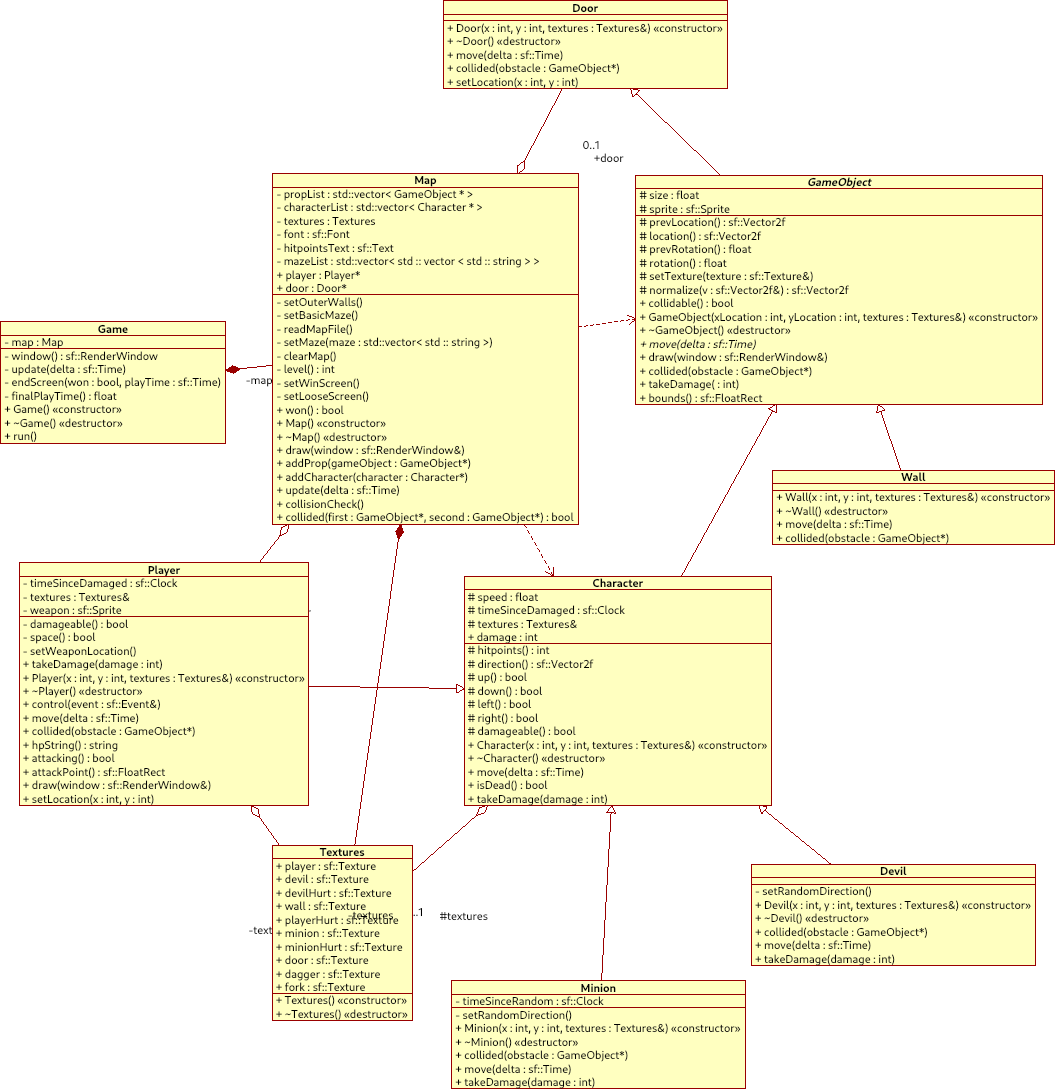
\includegraphics[scale=0.58]{uml-diagram}

\section{Detaljbeskrivning}
Två av mina klasser kan vara extra intressanta att analysera: Playerklassen och Mapklassen.

\subsection{Playerklassen}
Playerklassen ska representera spelaren. Klassen implementerar Characterklassen som i sin tur ärver från GameObjectklassen. \\
Playerklassen interagerar direkt med två klasser, Mapklassen och Texturesklassen. 
\subsubsection{Attribut}
Dessa attribut är specificerade i Characterklassen som i sin tur ärver av GameObjectklassen.
Jag diskuterar de mest intressanta.
\begin{itemize}
  \item sf::Sprite: sprite - sprite som representerar spelaren på spelplanen.
  \item sf::vector2f: location - positionen som spelaren har just nu.
  \item float: rotation - rotationen som spelarens sprite har.
  \item int: hitpoints - antalet liv spelaren har.
  \item float: speed - hur snabbt spelaren kan röra sig.
  \item int: damage - hur mycket skada spelaren gör när den attackerar.
  \item sf::Time: timeSinceDamaged - tiden sen spelaren sist blev skadad.
  \item sf::Sprite: weapon - spriten som representerar vapnet som spelaren använder.
\end{itemize}
\subsubsection{Metoder}
Playerklassen ärver många metoder av sina föräldrar. Men vissa är 'overload' med lite annorlunda funktionalitet.
Vissa metoder är lite extra intressanta.
\begin{itemize}
  \item attackPoint() - exponerar spelarens vapens position för att hantera kollisioner.
  \item control() - metod för att hantera knapptryckningar som styr spelaren.
  \item isDead() - kollar ifall spelaren är död, ärvd från Characterklassen.
\end{itemize}

\newpage

\subsection{Mapklassen}
Mapklassen representerar spelplanen. Spelplanen innehåller alla objekt som implementerar GameObjectklassen. \\
Mapklassen interagerar med GameObjectklassen för att kunna avgöra om en kollision har inträffat och för att 
uppdatera objektens positioner. Mapklassen ansvarar även för att bygga upp banan samt att läsa in 
spelplansfilerna. \\
\subsubsection{Attribut}
\begin{itemize}
  \item vector<GameObject>: propList - en vector av referenser till alla instanser av GameObjectklassen som inte är en Character. 
  i praktiken är det bara Wallklassen, men om något mer hinder skulle läggas till så ska samma vector kunna användas.
  \item vector<Character>: characterList - en vector av referenser till alla Characters, utom spelaren.
  \item Player: player - Referensen till spelaren. Då vi alltid interagerar med spelare så ligger den utanför vectorn för characters.
\end{itemize}
\subsubsection{Metoder}
Den viktigaste metoden i Mapklassen är collisionCheck().
\begin{itemize}
  \item collisionCheck() - metod för att se ifall en kollision har skett, den går igenom alla objekt och parar ihop dem en efter en 
  för att se ifall de har skett en kollistion. Det är inte en effektiv lösning men är den bästa jag kan komma på med de begränsningar jag har.
  \item update() - metoden som uppdaterar alla objekt. Den ändrar positioner, ser om något objekt ska förstöras och flyttar på de sprites som ska 
  flyttas på.
\end{itemize}


\newpage
\section{Diskussion}
I mitt spel så utgår allt från en instans av Gameklassen, Gameklassen innehåller en instans av Mapklassen. Gameklassen har även ansvaret att köra
spelloopen, som i sin tur kräver att Gameklassen håller koll på tiden mellan varje varv av loopen. 
Map-instansen innehåller alla GameObject-instanser, och har koll på om objekt har kolliderat.
Jag valde den här typen av design då det blir väldigt lätt att lägga till och ändra hur spelet ska se ut. \\
Om man till exempel vill lägga till andra hinder eller karaktärer så behöver vi inte ändra i de allra flesta klasser.
Kollisionshanteringen sker mellan spelobjekt så om vi skulle vilja ändra vad som händer vid kollision så ändrar vi bara i det spelobjektets klass.
Tanken är att minska coupling och ha hög cohesion.
Nackdelen är att varje 'tick' så måste Mapklassen kolla om varje GameObject krockar med alla andra GameObjects, 
så har man många GameObjects så kan spelet ta stora resurser. 
GameObjectklassen ärvs av flera klasser, och Mapklassen ska försöka att behandla alla typer som GameObjects, nackdelen är att nästan alla metoder 
som används i någon av klasserna måste finnas i GameObjectklassen, även om implementeringen är olika. Detta för att antalet metoder för till exempel 
Wallklassen är rätt många när Wallklassen egentligen bara använder några få.
Min arvstuktur har blivit 'fulare' på grund av hur SFML hanterar Textures, så jag behövde skapa en hjälpklass för just det och den refereras av 
nästan alla klasser. \\
Hade jag gjort om spelet hade jag nog inte försökt att få till en snygg arvsstruktur.

\section{Externa filformat}
Om vi bortser från png-filerna som bara är där för estetiska skäl så är det enda externa filformatet det för banorna.
Mitt spel använder sig av en enkel fil där specifikationen för banan är skiven i text, ett tecken för varje ruta med olika tecken för varje objekt.

\end{document}
